\chapter{Drag}

The very first computers were created to do calculations of how
artillery would fly when shot at different angles. The calculations
were similar to the ones you just did for the flying
hammer, with two important differences:
\begin{itemize}
\item They were interested in two dimensions: the height and the distance across the ground.
\item However, artillery flies a lot faster than a hammer, so they also had to worry about drag from the air.
\end{itemize}
\begin{figure}[htbp]
    \centering
    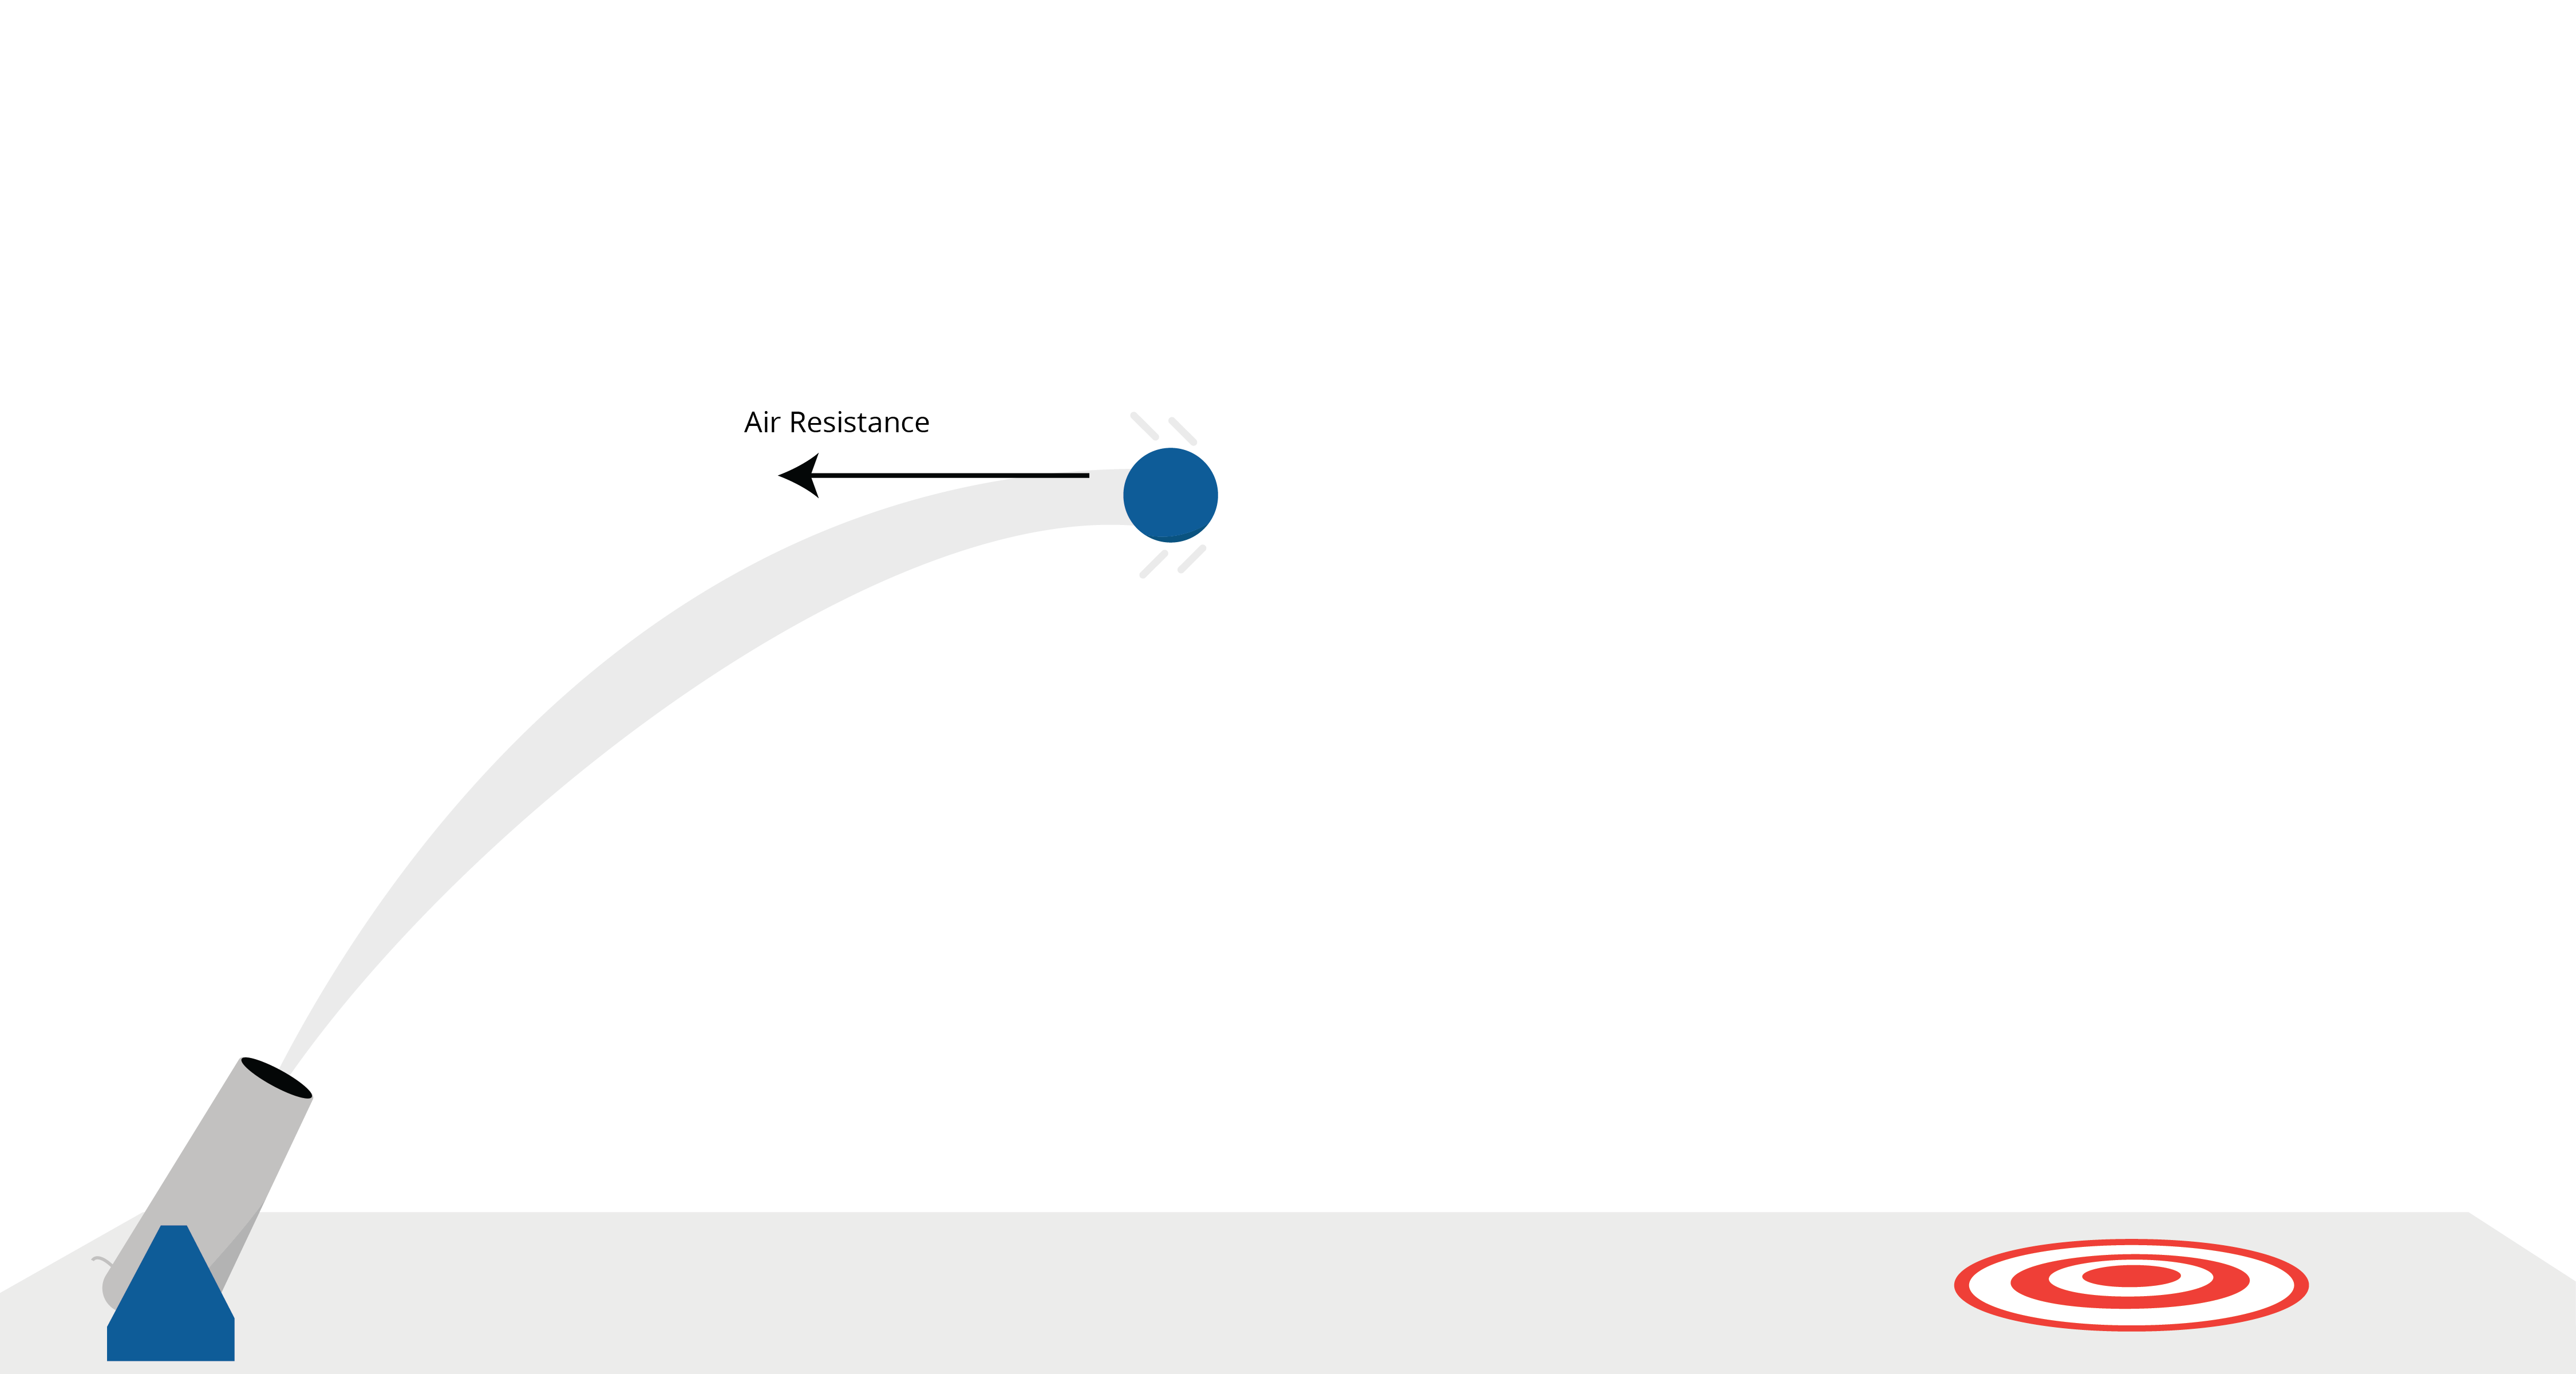
\includegraphics[width=1\textwidth]{cannon.png}
    \caption{A cannonball shot has a parabolic trajectory.}
    \label{fig:cannon}
\end{figure}
\section{Wind resistance}
\index{wind resistance}
The first thing they did was put one of the shells in a wind tunnel.
They measured how much force was created when they pushed 1 m/s of
wind over the shell. Let's say it was 0.1 newtons.

One of the interesting things about the drag from the air (often
called \newterm{wind resistance}) is that it increases with the
\emph{square} of the speed. Thus, if the wind pushing on the shell is
3 m/s, instead of 1 m/s, the resistance is $3^2 \times 0.1 = 0.9$
newtons.

(Why? Intuitively, three times as many air molecules are hitting the
shell and each molecule is hitting it three times harder.)

So, if a shell is moving with the velocity vector $v$, the force
vector of the drag points in the exact opposite direction. If $\mu$ is
the force of wind resistance of the shell at 1 m/s, then the magnitude
of the drag vector is $\mu |v|^2$ with $\mu$ being the wind resistance force.

\section{Initial velocity and acceleration due to gravity}

Let's say a shell is shot out of a tube at $s$ m/s, and the tube
is tilted $\theta$ radians above level. The initial velocity
will be given by the vector $[s \cos(\theta), s \sin(\theta)]$

\begin{figure}[htbp]
    \centering
    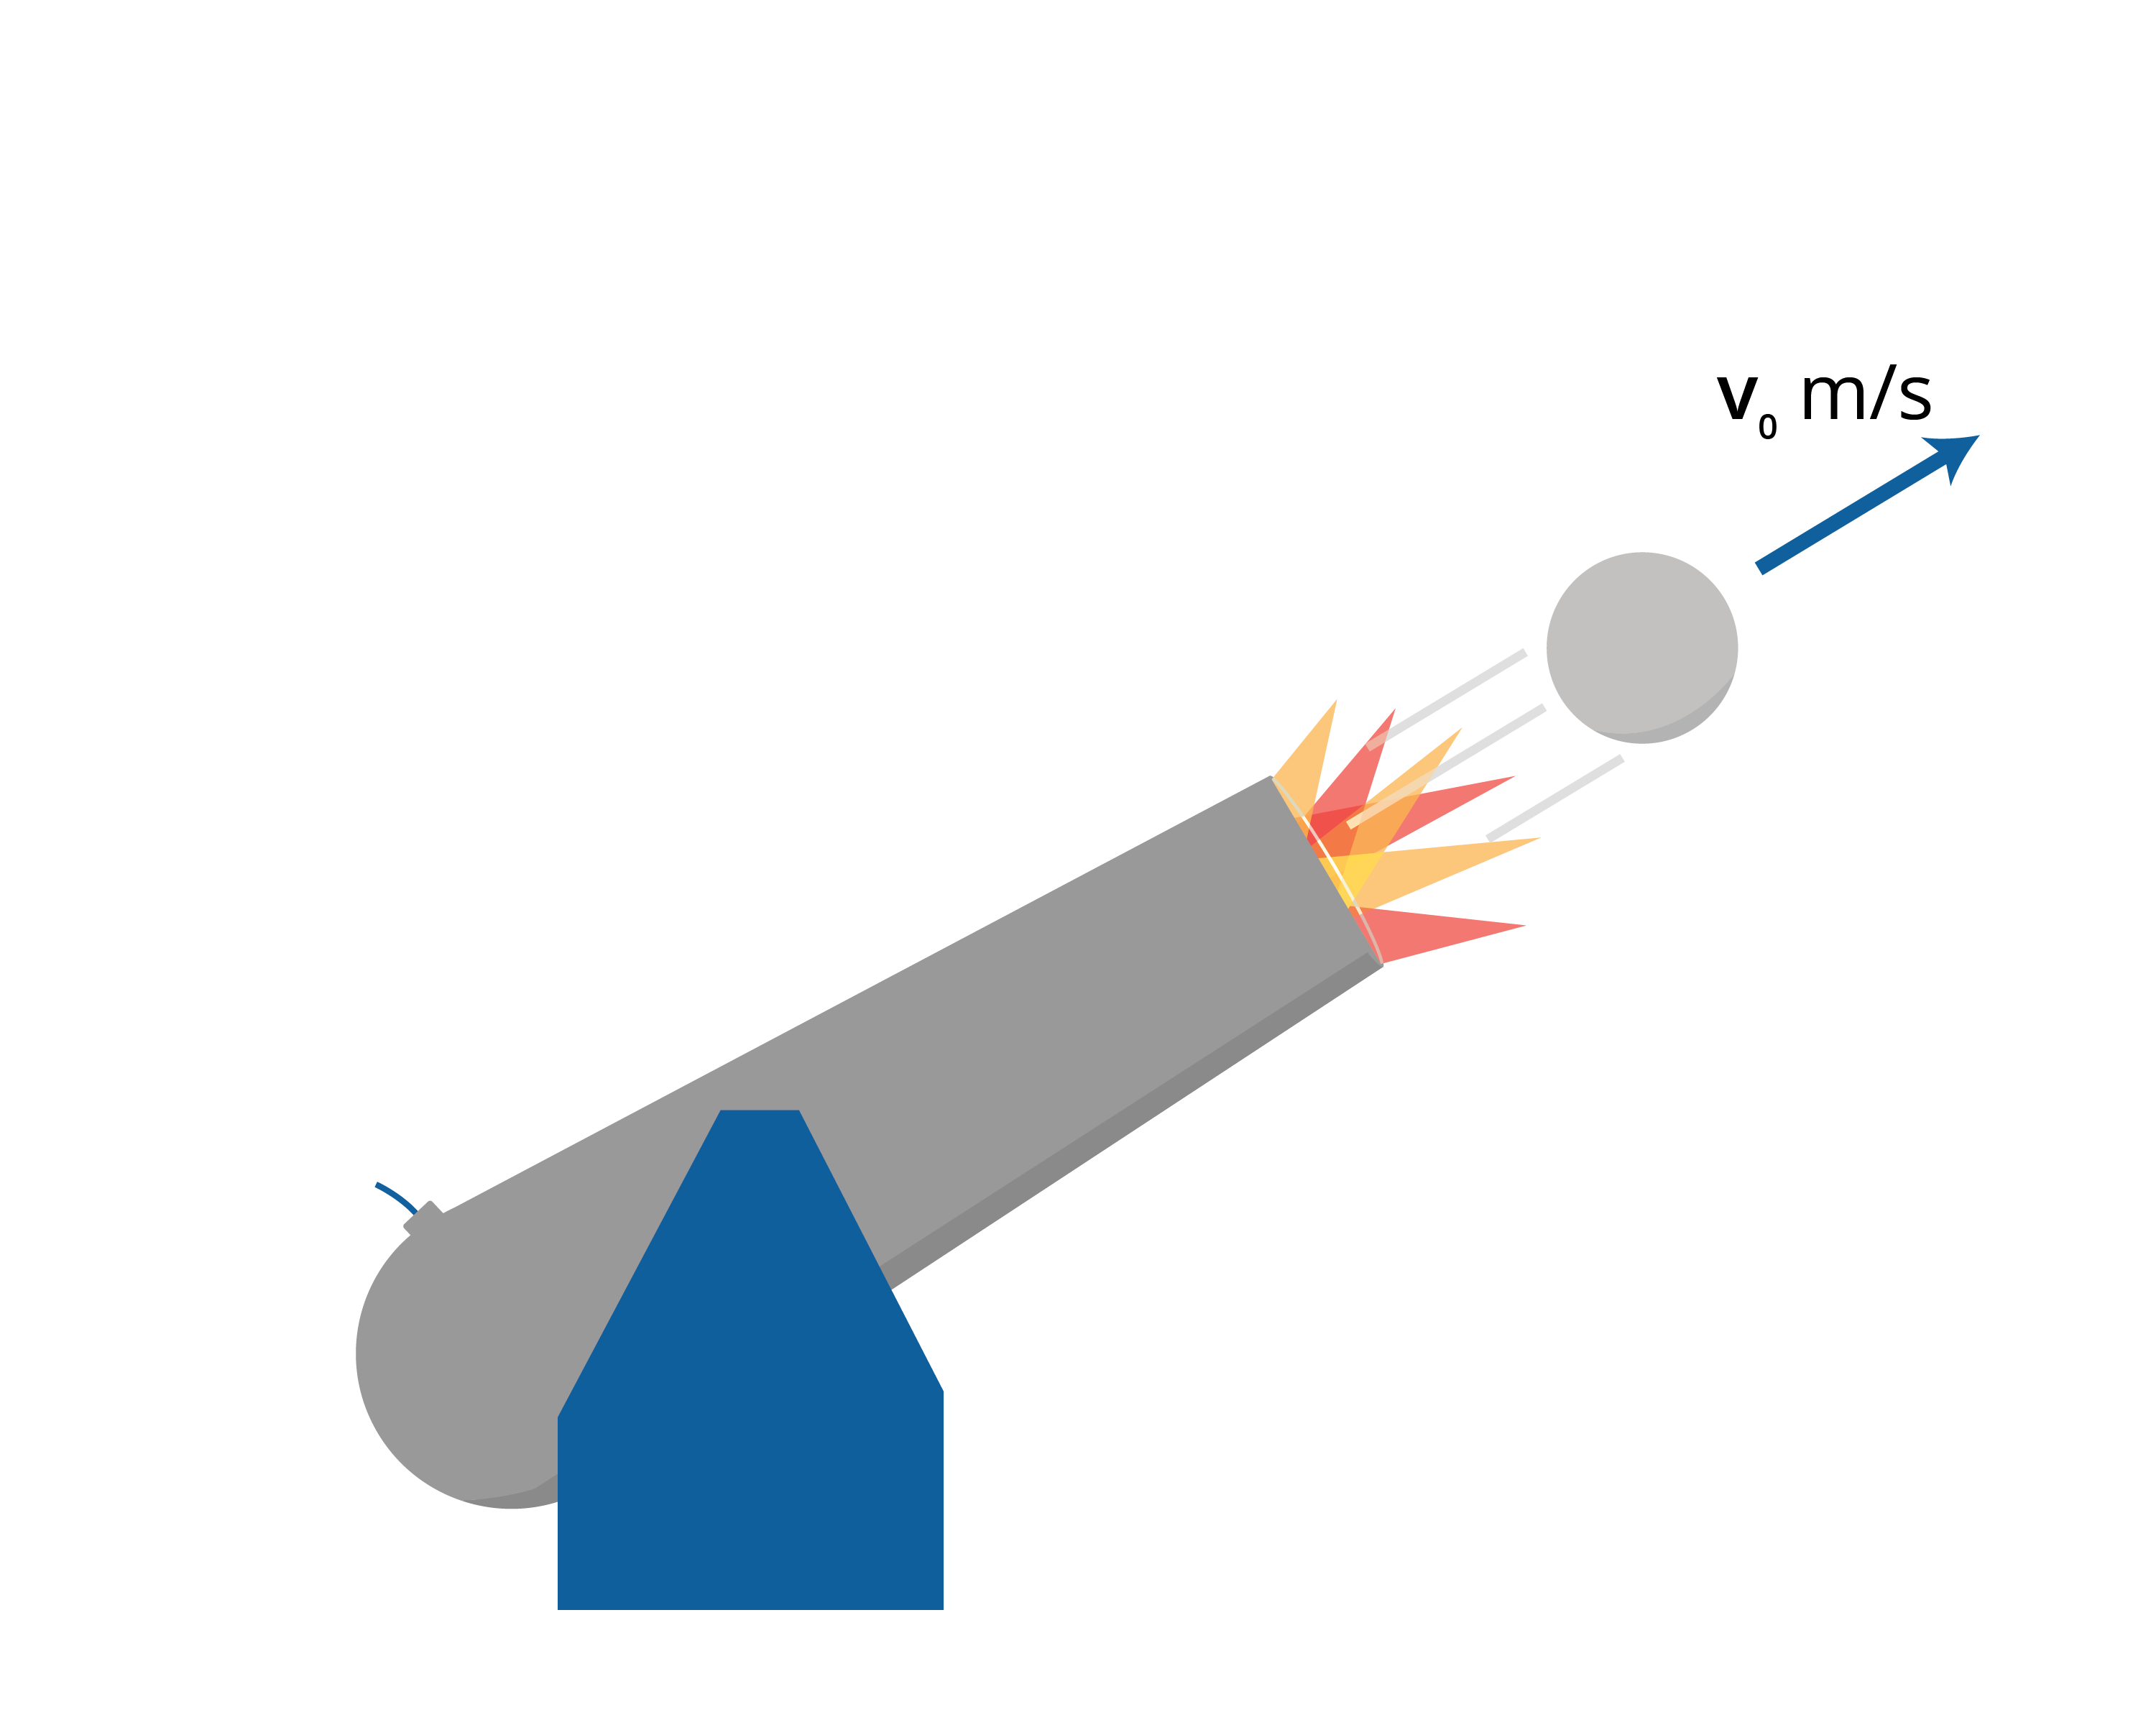
\includegraphics[width=.5\textwidth]{cannonvi.png}
    \caption{The initial velocity vector of the shell.}
    \label{fig:cannonvi}
\end{figure}



(The velocity of the shell is actually a 3-dimensional vector, but we
are only going to worry about height and horizontal distance; we are
assuming that the operator pointed it in the right direction.)

To figure out the path of the shell, we need to compute its acceleration. We remember that

$$F = m a$$

(Note that $F$ and $a$ are vectors.)  Dividing both sides by $m$, we get:

$$a = \frac{F}{m}$$

Let's figure out the net force on the shell, so that we can calculate the acceleration vector.

If the shell has a mass of $b$, the force due to gravity will be in the
downward direction, with a magnitude of $9.8 b$ newtons.

To get the net force, we will need to add the force due to gravity
with the force due to wind resistance.
%FIXME is this finished? seems like an odd stopping point
\section{Simulating artillery in Python}

Create a file called \filename{artillery.py}.

\begin{Verbatim}
    import numpy as np
    import matplotlib.pyplot as plt
    
    # Constants
    mass = 45 # kg
    start_speed = 300.0 # m/s
    theta = np.pi/5 # radians (36 degrees above level)
    time_step = 0.01 # s
    wind_resistance = 0.05 # newtons in 1 m/s wind
    force_of_gravity = np.array([0.0, -9.8 * mass]) # newtons
    
    # Initial state
    position = np.array([0.0, 0.0]) # [distance, height] in meters
    velocity = np.array([start_speed * np.cos(theta), start_speed * np.sin(theta)])
    time = 0.0 # seconds
    
    # Lists to gather data
    distances = []
    heights = []
    times = []
    
    # While shell is aloft
    while position[1] >= 0:
        # Record data
        distances.append(position[0])
        heights.append(position[1])
        times.append(time)
    
        # Calculate the next state
        time += time_step
        position += time_step * velocity
    
        # Calculate the net force vector
        force = force_of_gravity - wind_resistance * velocity**2
    
        # Calculate the current acceleration vector
        acceleration = force / mass
    
        # Update the velocity vector   
        velocity += time_step * acceleration
    
    print(f"Hit the ground {position[0]:.2f} meters away at {time:.2f} seconds.")
    
    # Plot the data
    fig, ax = plt.subplots()
    ax.plot(distances, heights)
    ax.set_title("Distance vs. Height")
    ax.set_xlabel("Distance (m)")
    ax.set_ylabel("Height (m)")
    plt.show()        
\end{Verbatim}

When you run it, you should get a message like:
\begin{Verbatim}
Hit the ground 1696.70 meters away at 20.73 seconds.
\end{Verbatim}

You should also see a plot of the shell's path:

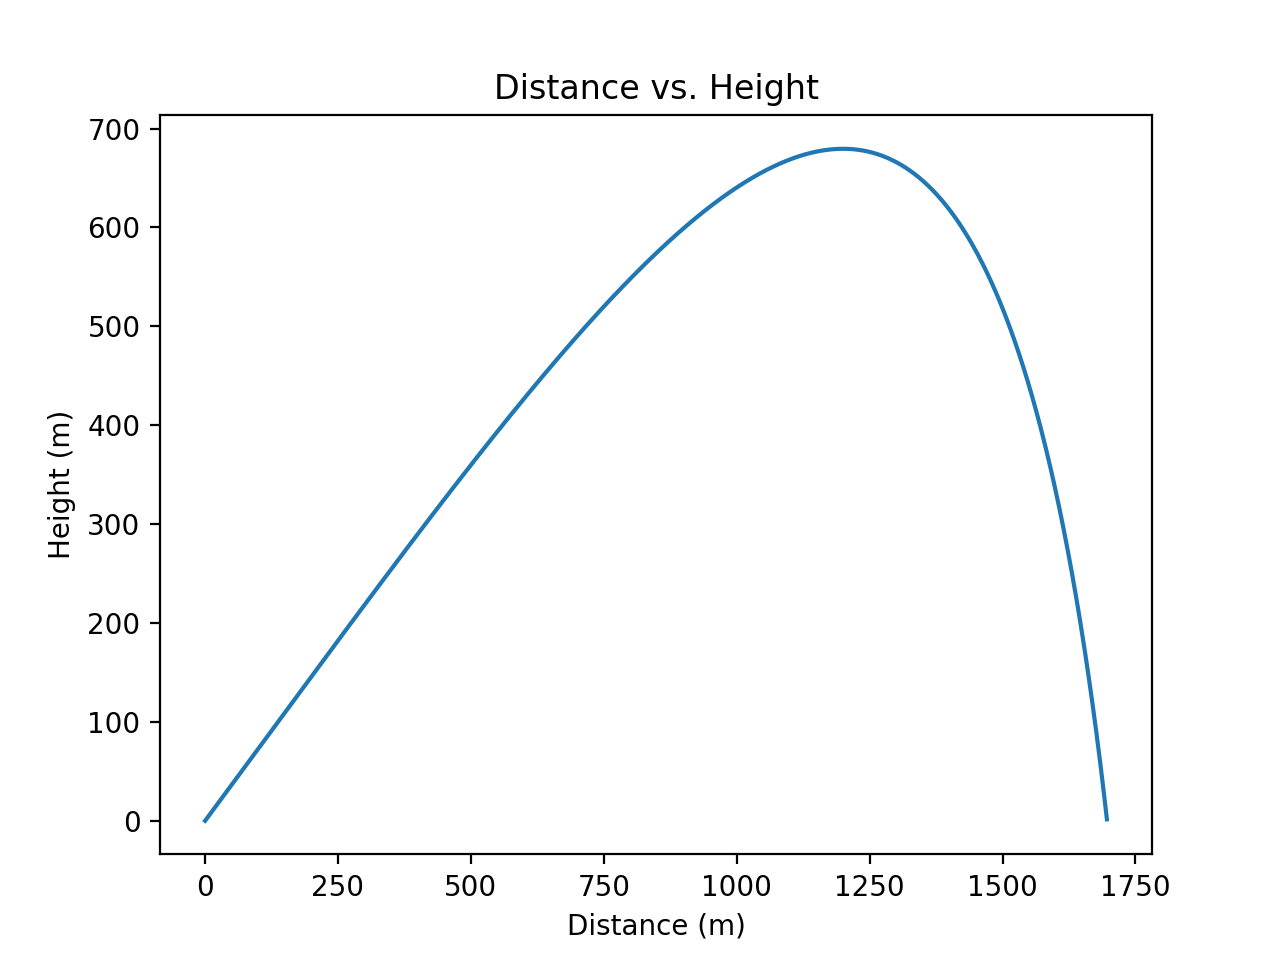
\includegraphics[width=0.8\textwidth]{artillery.png}

\section{Terminal velocity}
\index{terminal velocity}
If you shot the shell very, very high in the sky, it would keep accelerating 
toward the ground until the force of gravity and the force of the wind resistance were equal.
The speed at which this happens is called the \newterm{terminal velocity}.  The terminal velocity of a
falling human is about 53 m/s.
%FIXME expand 

Note that kinematic equations do not apply to terminal velocity, because the acceleration is not constant. Instead, we can use the fact that at terminal velocity, the force of wind resistance equals the force of gravity.
\begin{Exercise}[title={Terminal velocity}, label=terminal_velocity]
    What is the terminal velocity of the shell described in our example?
\end{Exercise}
\begin{Answer}[ref=terminal_velocity]
The force of gravity is $9.8 \times 45 = 441$ newtons.

At any speed $s$, the force of wind resistance is $0.05 \times s^2 = 0.05 s^2$ newtons.

At terminal velocity, $0.05 s^2 = 441$. 

Solving for $s$, we get $s = \sqrt{\frac{441}{0.05}}$

Thus, terminal velocity should be about 94 m/s.

\end{Answer}
